\documentclass{beamer}\usepackage[]{graphicx}\usepackage[]{xcolor}
% maxwidth is the original width if it is less than linewidth
% otherwise use linewidth (to make sure the graphics do not exceed the margin)
\makeatletter
\def\maxwidth{ %
  \ifdim\Gin@nat@width>\linewidth
    \linewidth
  \else
    \Gin@nat@width
  \fi
}
\makeatother

\definecolor{fgcolor}{rgb}{0.345, 0.345, 0.345}
\newcommand{\hlnum}[1]{\textcolor[rgb]{0.686,0.059,0.569}{#1}}%
\newcommand{\hlstr}[1]{\textcolor[rgb]{0.192,0.494,0.8}{#1}}%
\newcommand{\hlcom}[1]{\textcolor[rgb]{0.678,0.584,0.686}{\textit{#1}}}%
\newcommand{\hlopt}[1]{\textcolor[rgb]{0,0,0}{#1}}%
\newcommand{\hlstd}[1]{\textcolor[rgb]{0.345,0.345,0.345}{#1}}%
\newcommand{\hlkwa}[1]{\textcolor[rgb]{0.161,0.373,0.58}{\textbf{#1}}}%
\newcommand{\hlkwb}[1]{\textcolor[rgb]{0.69,0.353,0.396}{#1}}%
\newcommand{\hlkwc}[1]{\textcolor[rgb]{0.333,0.667,0.333}{#1}}%
\newcommand{\hlkwd}[1]{\textcolor[rgb]{0.737,0.353,0.396}{\textbf{#1}}}%
\let\hlipl\hlkwb

\usepackage{framed}
\makeatletter
\newenvironment{kframe}{%
 \def\at@end@of@kframe{}%
 \ifinner\ifhmode%
  \def\at@end@of@kframe{\end{minipage}}%
  \begin{minipage}{\columnwidth}%
 \fi\fi%
 \def\FrameCommand##1{\hskip\@totalleftmargin \hskip-\fboxsep
 \colorbox{shadecolor}{##1}\hskip-\fboxsep
     % There is no \\@totalrightmargin, so:
     \hskip-\linewidth \hskip-\@totalleftmargin \hskip\columnwidth}%
 \MakeFramed {\advance\hsize-\width
   \@totalleftmargin\z@ \linewidth\hsize
   \@setminipage}}%
 {\par\unskip\endMakeFramed%
 \at@end@of@kframe}
\makeatother

\definecolor{shadecolor}{rgb}{.97, .97, .97}
\definecolor{messagecolor}{rgb}{0, 0, 0}
\definecolor{warningcolor}{rgb}{1, 0, 1}
\definecolor{errorcolor}{rgb}{1, 0, 0}
\newenvironment{knitrout}{}{} % an empty environment to be redefined in TeX

\usepackage{alltt}					% Document class

\mode<presentation>
{
  \usetheme{default}                    % Set theme
  \usecolortheme{default}               % Set colors
  \usefonttheme{default}                % Set font theme
  \setbeamertemplate{caption}[numbered] % Set caption to be numbered
}

\usepackage{graphicx}  % For including figures
\usepackage{booktabs}  % For table rules
\usepackage{hyperref}  % For cross-referencing

\title{My Biography}  % Presentation title
\author{Frank Kusi Agyemang}                              % Presentation author
\institute{University of Nebraska-Lincoln}                  % Author affiliation
\date{\today}                                    % Today's date

% This creates a bibliography file with the same name as the main file.
% Mostly, it allows us to have only one text file to lug around.
\begin{filecontents}{\jobname.bib}
@article{healyFuckNuance2017,
	title = {Fuck {Nuance}},
	volume = {35},
	doi = {10.1177/0735275117709046},
	number = {2},
	journal = {Sociological Theory},
	author = {Healy, Kieran},
	month = jun,
	year = {2017},
	pages = {118--127}
}
@article{lego,
	title = {Everything is awesome: Don't forget the {Lego}},
	volume = {55},
	doi = {10.1111/jpc.14309},
	number = {8},
	journal = {Journal of Paediatrics and Child Health},
	author = {Tagg, Andrew and Roland, Damian and Leo, Grace SY and Knight, Katie and Goldstein, Henry and Davis, Tessa},
	year = {2019},
	pages = {921--923},
}
\end{filecontents}
\IfFileExists{upquote.sty}{\usepackage{upquote}}{}
\begin{document}
\SweaveOpts{concordance=TRUE}


\begin{frame}
  \titlepage 
\end{frame}


\begin{frame}{Outline}
  \tableofcontents 
\end{frame}

\section{Background}

\begin{frame}{About Me}
	My name is Frank Kusi Agyemang. I am from Ghana and currently a graduate student at the University of Nebraska-Lincoln, pursuing a Master of Science degree in Statistics. I am 23yrs old. I was born in Kumasi, the second largest city in Ghana. Additional things that I would add are my hobbies. Good food and good music.
\end{frame}

\section{Favorite Pets}

\begin{frame}{Favorite Pets}
\begin{itemize}
        \item Penguins
	\end{itemize}
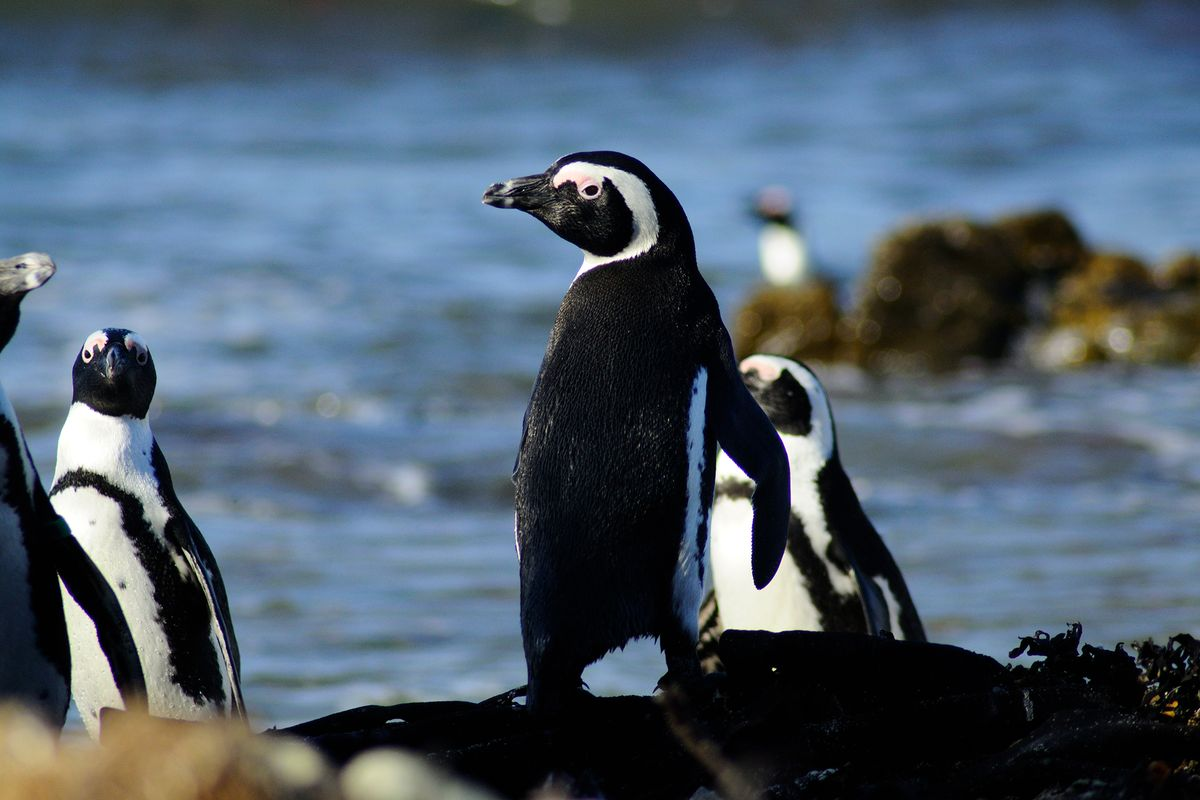
\includegraphics[scale=0.6]{penguin.png}
\end{frame}


\begin{frame}
\begin{itemize}
		\item Parrots
\end{itemize}
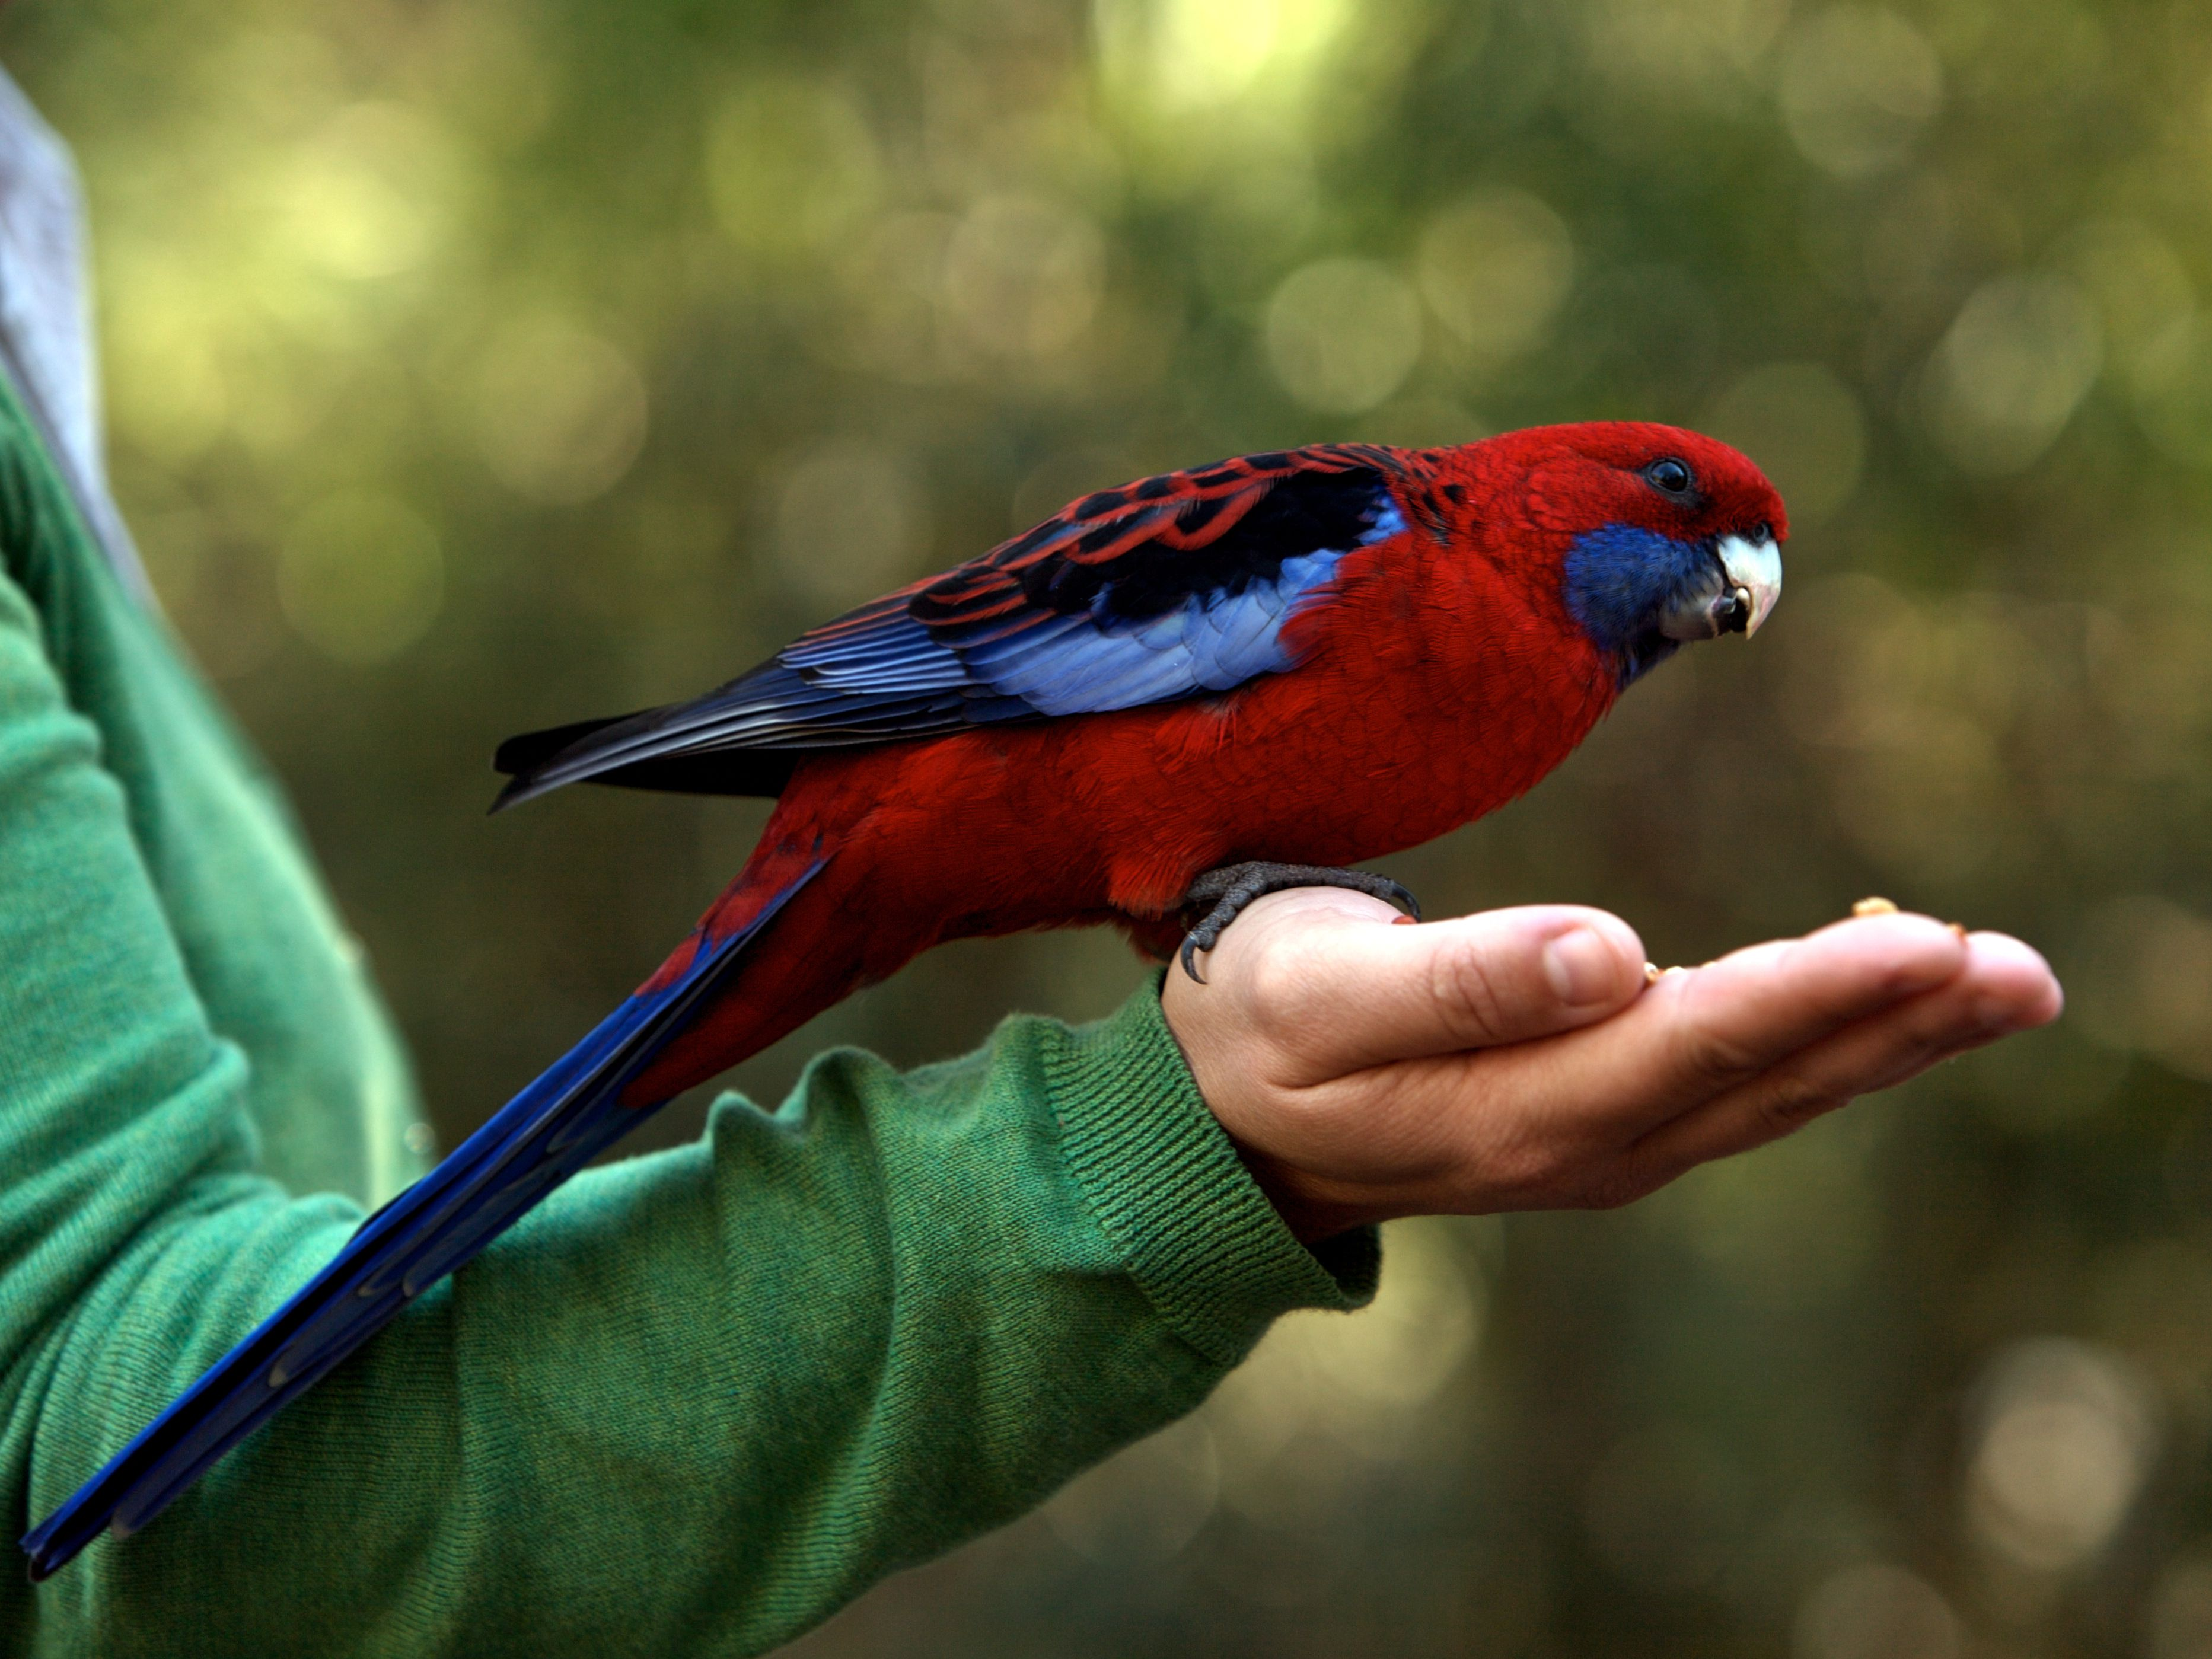
\includegraphics[scale=0.7]{parrots.png}

\end{frame}

\section{Graphs}






% Adding the option 'allowframebreaks' allows the contents of the slide to be expanded in more than one slide.
\begin{frame}[allowframebreaks]{References}
	\bibliography{\jobname}
	\bibliographystyle{apalike}
\end{frame}

\begin{frame}{graphics}
\begin{knitrout}
\definecolor{shadecolor}{rgb}{0.969, 0.969, 0.969}\color{fgcolor}\begin{kframe}
\begin{alltt}
\hlcom{#library(readr)}
\hlcom{#install.packages("ggplot2")}
\hlcom{# sessionInfo()}
\hlcom{# library(ggplot2)}
\hlcom{#library(tidyverse)}
\hlcom{#library(mclust)}
\hlcom{#library(purr)}
\hlcom{#library(stringr)}

\hlstd{penguins} \hlkwb{<-} \hlkwd{read.csv}\hlstd{(}\hlstr{"penguins.csv"}\hlstd{)}

\hlkwd{hist}\hlstd{(}\hlkwc{x}\hlstd{=penguins}\hlopt{$}\hlstd{bill_length_mm)}
\end{alltt}
\end{kframe}
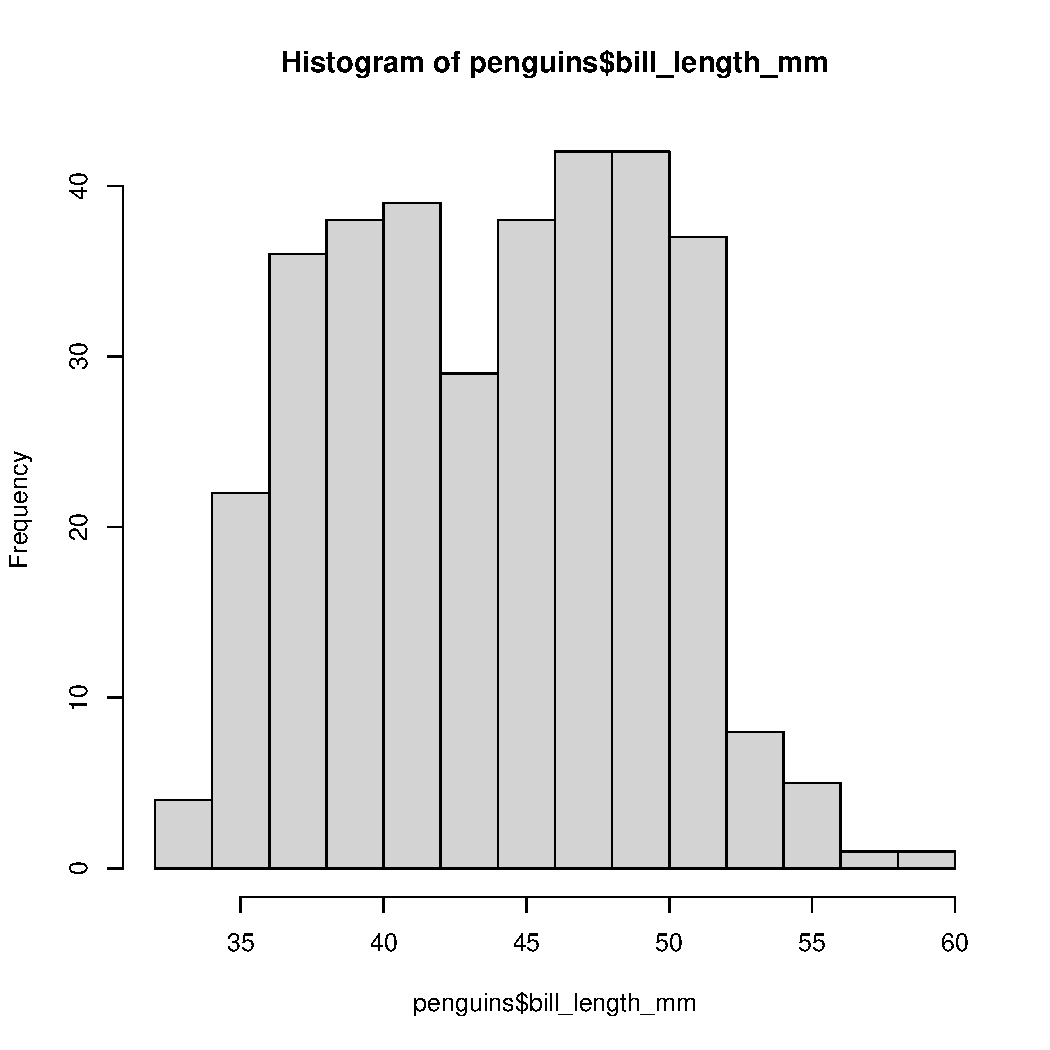
\includegraphics[width=\maxwidth]{figure/unnamed-chunk-1-1} 
\begin{kframe}\begin{alltt}
\hlcom{# ggplot(data = penguins, mapping = aes(x = "bill_length_mm", y = "bill_depth_mm")) + geom_hist(color = "red", alpha = .5, size = 4, shape = 6)+ ggtitle("2021 NTSE Endowment Market Values US and Canadian Institutions--REVISED March 1 2022")}
\end{alltt}
\end{kframe}
\end{knitrout}
\end{frame}

\end{document}
